% Drawing 154/06-18 -- folder 154, batch 06, archive page 120 (PDF page 121).
% Transcription: sur une feuille de listing imprimée (bannière de travail), des croquis : en haut, en couleur, un ruban vert foncé fermé autour d'une droite noircie, traversé par deux paires de droites rouges ; ailleurs, au crayon, des droites qui se croisent deux à deux sur une droite fléchée, un parallélépipède en perspective, des quadrilatères aux sommets marqués d'un point et des ovales traversés de droites
% Kind: ribbon round a blackened line crossed by two pairs of lines; pencil sketches. Method 2 (schematic redraw from the facsimile). Status: partial.
% Notes: On a printed listing (CRAY2 job banner, 16 Aug 82; not reproduced). Top, in colour: a dark green ribbon closed round a blackened line, crossed by two pairs of red lines. Elsewhere in pencil, drawn in part: lines crossing two by two on an arrowed line, a parallelepiped in perspective, quadrilaterals with vertices marked by a point, and ovals crossed by lines (one oval and a few crossings drawn). Read from the page view.
% Coordinates: 1 unit = 1 mm = 1/100 of the crop width (bbox in page fractions: [0.152, 0.076, 0.964, 0.499]).
% Redrawn by Claude (claude-opus-5-5), issue #73, 2026-11-07; not checked by a human; not compiled (no TeX in the session).
% Rights: reproduces part of the work -- behind RENDER_TRANSCRIPTS, never published by itself.
\documentclass[tikz,border=3pt]{standalone}
\usepackage{amsmath,amssymb}
\usetikzlibrary{patterns,arrows.meta}
\tikzset{Or/.style={orange!90!black}, Ye/.style={yellow!80!orange}, Lg/.style={green!60!black!70}, Dg/.style={green!45!black}, Br/.style={brown!80!black}, Rd/.style={red!85!black}, Bl/.style={blue!70!black}, Gy/.style={black!40}, pencil/.style={black!45}, struck/.style={black!35}, mark/.style={circle,draw,inner sep=1.3pt}, pt/.style={circle,fill,inner sep=0.9pt}, opt/.style={circle,draw,fill=white,inner sep=1.1pt}}
\begin{document}
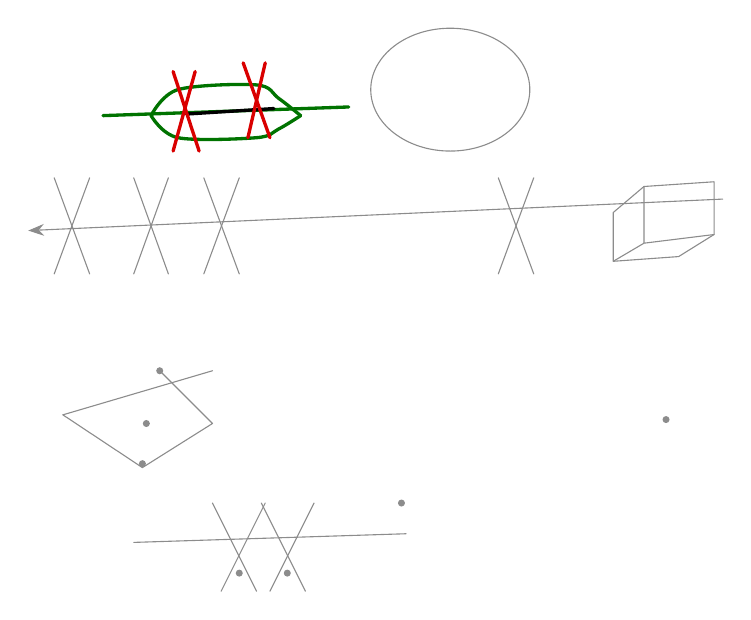
\begin{tikzpicture}[x=1mm,y=1mm,line cap=round,line join=round,font=\scriptsize]
\draw[Dg,very thick] (10.1,-11.7) -- (41.3,-10.6);
\draw[Dg,very thick] plot[smooth, tension=0.55] coordinates {(16.2,-11.7) (19.6,-8.4) (29.6,-7.8) (32.4,-9.5) (35.2,-11.7)};
\draw[Dg,very thick] plot[smooth, tension=0.55] coordinates {(16.2,-11.7) (19.6,-14.5) (29.6,-14.5) (32.4,-13.4) (35.2,-11.7)};
\draw[very thick] (20.7,-11.5) -- (31.8,-10.8);
\draw[Rd,very thick] (19,-6.1) -- (22.3,-16.2);
\draw[Rd,very thick] (21.8,-6.1) -- (19,-16.2);
\draw[Rd,very thick] (27.9,-5) -- (31.3,-14.5);
\draw[Rd,very thick] (30.7,-5) -- (28.5,-14.5);
\draw[pencil,-{Stealth[length=2mm]}] (88.8,-22.3) -- (0.6,-26.3);
\draw[pencil] (3.9,-19.6) -- (8.4,-31.8);
\draw[pencil] (8.4,-19.6) -- (3.9,-31.8);
\draw[pencil] (14,-19.6) -- (18.4,-31.8);
\draw[pencil] (18.4,-19.6) -- (14,-31.8);
\draw[pencil] (22.9,-19.6) -- (27.4,-31.8);
\draw[pencil] (27.4,-19.6) -- (22.9,-31.8);
\draw[pencil] (60.3,-19.6) -- (64.8,-31.8);
\draw[pencil] (64.8,-19.6) -- (60.3,-31.8);
\draw[pencil] (74.9,-24) -- (78.8,-20.7) -- (87.7,-20.1) -- (87.7,-26.8) -- (83.2,-29.6) -- (74.9,-30.2) -- cycle;
\draw[pencil] (78.8,-20.7) -- (78.8,-27.9) -- (87.7,-26.8);
\draw[pencil] (78.8,-27.9) -- (74.9,-30.2);
\draw[pencil] (54.2,-8.4) ellipse[x radius=10.1, y radius=7.8];
\draw[pencil] (5,-49.7) -- (24,-44.1);
\draw[pencil] (5,-49.7) -- (15.1,-56.4);
\draw[pencil] (15.1,-56.4) -- (24,-50.8) -- (17.3,-44.1);
\node[pt,pencil] at (17.3,-44.1) {};
\node[pt,pencil] at (15.6,-50.8) {};
\node[pt,pencil] at (15.1,-55.9) {};
\node[pt,pencil] at (81.6,-50.3) {};
\node[pt,pencil] at (48,-60.9) {};
\node[pt,pencil] at (27.4,-69.8) {};
\node[pt,pencil] at (33.5,-69.8) {};
\draw[pencil] (24,-60.9) -- (29.6,-72.1);
\draw[pencil] (30.7,-60.9) -- (25.1,-72.1);
\draw[pencil] (30.2,-60.9) -- (35.8,-72.1);
\draw[pencil] (36.9,-60.9) -- (31.3,-72.1);
\draw[pencil] (14,-65.9) -- (48.6,-64.8);
\end{tikzpicture}
\end{document}
